\documentclass[]{article}
\usepackage{lmodern}
\usepackage{amssymb,amsmath}
\usepackage{ifxetex,ifluatex}
\usepackage{fixltx2e} % provides \textsubscript
\ifnum 0\ifxetex 1\fi\ifluatex 1\fi=0 % if pdftex
  \usepackage[T1]{fontenc}
  \usepackage[utf8]{inputenc}
\else % if luatex or xelatex
  \ifxetex
    \usepackage{mathspec}
  \else
    \usepackage{fontspec}
  \fi
  \defaultfontfeatures{Ligatures=TeX,Scale=MatchLowercase}
\fi
% use upquote if available, for straight quotes in verbatim environments
\IfFileExists{upquote.sty}{\usepackage{upquote}}{}
% use microtype if available
\IfFileExists{microtype.sty}{%
\usepackage{microtype}
\UseMicrotypeSet[protrusion]{basicmath} % disable protrusion for tt fonts
}{}
\usepackage[margin=1in]{geometry}
\usepackage{hyperref}
\hypersetup{unicode=true,
            pdftitle={閸掆晝鏁ゆ妯虹棄閸︽澘娴楢PI閻㈢喐鍨氱悰灞炬杺閸栧搫鍨濋崶},
            pdfauthor={閸涖劌宸},
            pdfborder={0 0 0},
            breaklinks=true}
\urlstyle{same}  % don't use monospace font for urls
\usepackage{color}
\usepackage{fancyvrb}
\newcommand{\VerbBar}{|}
\newcommand{\VERB}{\Verb[commandchars=\\\{\}]}
\DefineVerbatimEnvironment{Highlighting}{Verbatim}{commandchars=\\\{\}}
% Add ',fontsize=\small' for more characters per line
\usepackage{framed}
\definecolor{shadecolor}{RGB}{248,248,248}
\newenvironment{Shaded}{\begin{snugshade}}{\end{snugshade}}
\newcommand{\KeywordTok}[1]{\textcolor[rgb]{0.13,0.29,0.53}{\textbf{#1}}}
\newcommand{\DataTypeTok}[1]{\textcolor[rgb]{0.13,0.29,0.53}{#1}}
\newcommand{\DecValTok}[1]{\textcolor[rgb]{0.00,0.00,0.81}{#1}}
\newcommand{\BaseNTok}[1]{\textcolor[rgb]{0.00,0.00,0.81}{#1}}
\newcommand{\FloatTok}[1]{\textcolor[rgb]{0.00,0.00,0.81}{#1}}
\newcommand{\ConstantTok}[1]{\textcolor[rgb]{0.00,0.00,0.00}{#1}}
\newcommand{\CharTok}[1]{\textcolor[rgb]{0.31,0.60,0.02}{#1}}
\newcommand{\SpecialCharTok}[1]{\textcolor[rgb]{0.00,0.00,0.00}{#1}}
\newcommand{\StringTok}[1]{\textcolor[rgb]{0.31,0.60,0.02}{#1}}
\newcommand{\VerbatimStringTok}[1]{\textcolor[rgb]{0.31,0.60,0.02}{#1}}
\newcommand{\SpecialStringTok}[1]{\textcolor[rgb]{0.31,0.60,0.02}{#1}}
\newcommand{\ImportTok}[1]{#1}
\newcommand{\CommentTok}[1]{\textcolor[rgb]{0.56,0.35,0.01}{\textit{#1}}}
\newcommand{\DocumentationTok}[1]{\textcolor[rgb]{0.56,0.35,0.01}{\textbf{\textit{#1}}}}
\newcommand{\AnnotationTok}[1]{\textcolor[rgb]{0.56,0.35,0.01}{\textbf{\textit{#1}}}}
\newcommand{\CommentVarTok}[1]{\textcolor[rgb]{0.56,0.35,0.01}{\textbf{\textit{#1}}}}
\newcommand{\OtherTok}[1]{\textcolor[rgb]{0.56,0.35,0.01}{#1}}
\newcommand{\FunctionTok}[1]{\textcolor[rgb]{0.00,0.00,0.00}{#1}}
\newcommand{\VariableTok}[1]{\textcolor[rgb]{0.00,0.00,0.00}{#1}}
\newcommand{\ControlFlowTok}[1]{\textcolor[rgb]{0.13,0.29,0.53}{\textbf{#1}}}
\newcommand{\OperatorTok}[1]{\textcolor[rgb]{0.81,0.36,0.00}{\textbf{#1}}}
\newcommand{\BuiltInTok}[1]{#1}
\newcommand{\ExtensionTok}[1]{#1}
\newcommand{\PreprocessorTok}[1]{\textcolor[rgb]{0.56,0.35,0.01}{\textit{#1}}}
\newcommand{\AttributeTok}[1]{\textcolor[rgb]{0.77,0.63,0.00}{#1}}
\newcommand{\RegionMarkerTok}[1]{#1}
\newcommand{\InformationTok}[1]{\textcolor[rgb]{0.56,0.35,0.01}{\textbf{\textit{#1}}}}
\newcommand{\WarningTok}[1]{\textcolor[rgb]{0.56,0.35,0.01}{\textbf{\textit{#1}}}}
\newcommand{\AlertTok}[1]{\textcolor[rgb]{0.94,0.16,0.16}{#1}}
\newcommand{\ErrorTok}[1]{\textcolor[rgb]{0.64,0.00,0.00}{\textbf{#1}}}
\newcommand{\NormalTok}[1]{#1}
\usepackage{graphicx,grffile}
\makeatletter
\def\maxwidth{\ifdim\Gin@nat@width>\linewidth\linewidth\else\Gin@nat@width\fi}
\def\maxheight{\ifdim\Gin@nat@height>\textheight\textheight\else\Gin@nat@height\fi}
\makeatother
% Scale images if necessary, so that they will not overflow the page
% margins by default, and it is still possible to overwrite the defaults
% using explicit options in \includegraphics[width, height, ...]{}
\setkeys{Gin}{width=\maxwidth,height=\maxheight,keepaspectratio}
\IfFileExists{parskip.sty}{%
\usepackage{parskip}
}{% else
\setlength{\parindent}{0pt}
\setlength{\parskip}{6pt plus 2pt minus 1pt}
}
\setlength{\emergencystretch}{3em}  % prevent overfull lines
\providecommand{\tightlist}{%
  \setlength{\itemsep}{0pt}\setlength{\parskip}{0pt}}
\setcounter{secnumdepth}{0}
% Redefines (sub)paragraphs to behave more like sections
\ifx\paragraph\undefined\else
\let\oldparagraph\paragraph
\renewcommand{\paragraph}[1]{\oldparagraph{#1}\mbox{}}
\fi
\ifx\subparagraph\undefined\else
\let\oldsubparagraph\subparagraph
\renewcommand{\subparagraph}[1]{\oldsubparagraph{#1}\mbox{}}
\fi

%%% Use protect on footnotes to avoid problems with footnotes in titles
\let\rmarkdownfootnote\footnote%
\def\footnote{\protect\rmarkdownfootnote}

%%% Change title format to be more compact
\usepackage{titling}

% Create subtitle command for use in maketitle
\newcommand{\subtitle}[1]{
  \posttitle{
    \begin{center}\large#1\end{center}
    }
}

\setlength{\droptitle}{-2em}
  \title{閸掆晝鏁ゆ妯虹棄閸︽澘娴楢PI閻㈢喐鍨氱悰灞炬杺閸栧搫鍨濋崶}
  \pretitle{\vspace{\droptitle}\centering\huge}
  \posttitle{\par}
  \author{閸涖劌宸}
  \preauthor{\centering\large\emph}
  \postauthor{\par}
  \predate{\centering\large\emph}
  \postdate{\par}
  \date{2018楠\textless{}9e\textgreater{}3閺\textless{}88\textgreater{}\textless{}88\textgreater{}15閺\textless{}83\textgreater{}}


\begin{document}
\maketitle

\subsubsection{介绍}

在利用地图开展各种分析或制图时,准确的行政区划底图往往是不可或缺的。但由于我国目前行政区划(特别是区县级)调整比较频繁,互联网上的免费资源通常比较陈旧,只用这样的底图往往就不能准确反映现实情况了。好在高德地图提供了行政区域查询的WEB服务API\href{http://lbs.amap.com/api/webservice/guide/api/district/}{接口},可以通过这个接口查询我国各级行政区的行政区划地理空间信息,并利用返回的点坐标生成各级行政区划图。这样就可以利用高德地图的数据生产比较新的行政区划图了,而且高德说是``\textbf{唯一能让用户查询到乡镇/街道级别信息且小时级更新数据的公开API}''。惊喜不惊喜,意外不意外?废话不多说,下面我们就用R语言来即时生成行政区划底图吧。

\subsubsection{抓取信息}

\begin{Shaded}
\begin{Highlighting}[]
\KeywordTok{library}\NormalTok{(}\StringTok{'httr'}\NormalTok{)}
\KeywordTok{library}\NormalTok{(}\StringTok{'jsonlite'}\NormalTok{)}
\KeywordTok{library}\NormalTok{(}\StringTok{'tidyverse'}\NormalTok{)}
\KeywordTok{library}\NormalTok{(}\StringTok{'rlist'}\NormalTok{)}
\KeywordTok{library}\NormalTok{(}\StringTok{'Rgctc2'}\NormalTok{,}\DataTypeTok{lib.loc=}\StringTok{'~/GitHub/R_coordination_transformation'}\NormalTok{)}
\KeywordTok{library}\NormalTok{(}\StringTok{'sf'}\NormalTok{)}
\end{Highlighting}
\end{Shaded}

首先自然是写抓取信息的函数,利用高德的官方指南很容易搞定。

\begin{Shaded}
\begin{Highlighting}[]
\KeywordTok{options}\NormalTok{(}\DataTypeTok{digits=}\DecValTok{11}\NormalTok{)}
\NormalTok{get_location<-}\StringTok{ }\ControlFlowTok{function}\NormalTok{(address)\{}
\NormalTok{  key =}\StringTok{ '7c6b6c0d1b641f4aa9cdb7d2229ae728'}                            \CommentTok{#需要预先申请一个高德API的key}
\NormalTok{  url =}\StringTok{ 'http://restapi.amap.com/v3/config/district?'} \OperatorTok
\StringTok{        }\KeywordTok{paste}\NormalTok{(}\StringTok{'keywords='}\NormalTok{ , address ,}
              \StringTok{'&key='}\NormalTok{ ,key ,}
              \StringTok{'&subdistrict=1'}\NormalTok{ ,                                      }\CommentTok{#可以指定返回行政区的层级}
              \StringTok{'&extensions=all'}\NormalTok{,}
               \DataTypeTok{sep =} \StringTok{''}\NormalTok{)}
\NormalTok{  geoinfo<-}\KeywordTok{GET}\NormalTok{(url)}\OperatorTok\StringTok{ }\KeywordTok{content}\NormalTok{(}\DataTypeTok{as=}\StringTok{"text"}\NormalTok{,}\DataTypeTok{encoding=}\StringTok{"UTF-8"}\NormalTok{) }\OperatorTok\StringTok{ }
\StringTok{        }\KeywordTok{fromJSON}\NormalTok{(}\DataTypeTok{flatten =} \OtherTok{TRUE}\NormalTok{)                                      }\CommentTok{#返回信息的类型是可以选择的                    }
  \KeywordTok{return}\NormalTok{(geoinfo)}
\NormalTok{\}}
\end{Highlighting}
\end{Shaded}

这个爬虫就只需要一个参数\emph{address},支持中文地名,也支持数字形式的区域编码(adcode)。用中文地名查询时到了市、县这个层级就有可能碰到多义性的问题了,也就是一个关键字对应多个区域的情况,高德建议大家尽量使用adcode,可以在\href{http://lbs.amap.com/api/webservice/download}{这里}下载。我们可以通过上级行政区域获得所有下级行政区域的adcode,非常简单,可以用这个机制直接抓取指定行政区里所有下级行政区的adcode。值得一提的是预定设定小数点位数\texttt{options(digits=11)}。由于地理坐标小数点后的位数比较多,如果不预先指定小数点位数的话,按照R默认的精度就会出现显示不完整的情况。下面,我们赶紧来拿浙江做个例子吧。

\begin{Shaded}
\begin{Highlighting}[]
\NormalTok{   zj<-}\KeywordTok{get_location}\NormalTok{(}\StringTok{'浙江省'}\NormalTok{) }\OperatorTok\StringTok{ '[['}\NormalTok{(}\StringTok{'districts'}\NormalTok{)}
\end{Highlighting}
\end{Shaded}

返回的信息是一个包含了六个元素的列表,这个列表的\emph{districts}元素包含了我所需要的所有信息,所以这里就直接一步提取出来了,有兴趣的小伙伴可以自己查看返回列表的信息。下面我们就来看看这个\emph{districts}元素长什么样子吧。

\begin{verbatim}
## 'data.frame':    1 obs. of  7 variables:
##  $ citycode :List of 1
##   ..$ : list()
##  $ adcode   : chr "330000"
##  $ name     : chr "浙江省"
##  $ polyline : chr "121.134149,27.786010;121.134130,27.785898;121.134110,27.785840;121.134079,27.785817;121.134009,27.785782;121.13"| __truncated__
##  $ center   : chr "120.152585,30.266597"
##  $ level    : chr "province"
##  $ districts:List of 1
##   ..$ :'data.frame': 11 obs. of  6 variables:
##   .. ..$ citycode : chr  "0572" "0571" "0573" "0579" ...
##   .. ..$ adcode   : chr  "330500" "330100" "330400" "330700" ...
##   .. ..$ name     : chr  "湖州市" "杭州市" "嘉兴市" "金华市" ...
##   .. ..$ center   : chr  "120.086809,30.89441" "120.209789,30.24692" "120.75547,30.746191" "119.647229,29.079208" ...
##   .. ..$ level    : chr  "city" "city" "city" "city" ...
##   .. ..$ districts:List of 11
##   .. .. ..$ : list()
##   .. .. ..$ : list()
##   .. .. ..$ : list()
##   .. .. ..$ : list()
##   .. .. ..$ : list()
##   .. .. ..$ : list()
##   .. .. ..$ : list()
##   .. .. ..$ : list()
##   .. .. ..$ : list()
##   .. .. ..$ : list()
##   .. .. ..$ : list()
\end{verbatim}

为了比较清晰的展示数据结构,我选择只返回了下一级行政区的信息(\texttt{subdistrict=1}),也就是浙江的地级市信息。在实际中我设定\texttt{subdistrict=3},可以一步返回浙江所有镇的信息。
\emph{polyline}这个元素里就是我们要找的行政区边界上的坐标点的信息,目前是一个很长的字符串,后面主要的工作其实就是分割------转换类型------转换坐标系------生成地理空间对象,然后就可以作图啦。下面,我们就来处理浙江省的边界。

\subsubsection{清洗、转换}

\begin{verbatim}
##  chr "121.134149,27.786010;121.134130,27.785898;121.134110,27.785840;121.134079,27.785817;121.134009,27.785782;121.13"| __truncated__
\end{verbatim}

老规矩,先来看看\emph{polyline}的结构。类型,字符串型(chr);坐标是以经纬度的形式记录的,经纬度之间用\textbf{``,''}分隔,而每对坐标之间用\textbf{``;''}分隔。在后面,我们还看到了一个分隔符号\textbf{``\textbar{}''},这是什么意思呢?这表示着行政区并非只包括一个多边形。由于岛屿、飞地等类型的行政区,一个省的行政区可能会包括很多的独立多边形。每一个多边形之间都是用\textbf{``\textbar{}''}来分隔。了解清楚了数据结构,就可以开始进行分割和转换了。下面给出代码。

\begin{Shaded}
\begin{Highlighting}[]
\NormalTok{zj}\OperatorTok{$}\NormalTok{polyline<-zj}\OperatorTok{$}\NormalTok{polyline }\OperatorTok\StringTok{ }
\StringTok{             }\KeywordTok{str_split}\NormalTok{(}\StringTok{'}\CharTok{\textbackslash{}\textbackslash{}}\StringTok{|'}\NormalTok{) }\OperatorTok\StringTok{ }
\StringTok{             }\KeywordTok{lapply}\NormalTok{(str_split,}\StringTok{';'}\NormalTok{) }\OperatorTok\StringTok{ }
\StringTok{             '[['}\NormalTok{(}\DecValTok{1}\NormalTok{)}\OperatorTok\StringTok{ }\KeywordTok{lapply}\NormalTok{(str_split,}\StringTok{','}\NormalTok{) }\OperatorTok\StringTok{     }\CommentTok{#以上对字符串进行分隔,得到一个多层嵌套的列表            }
\StringTok{             }\KeywordTok{lapply}\NormalTok{(lapply,as.numeric) }\OperatorTok\StringTok{      }
\StringTok{             }\KeywordTok{lapply}\NormalTok{(list.rbind)}\OperatorTok\StringTok{                    }\CommentTok{#转换数据类型,并合并行,形成若干矩阵。}
\StringTok{  }
\StringTok{             }\KeywordTok{lapply}\NormalTok{(gcj02_wgs84_matrix_matrix) }\OperatorTok\StringTok{    }\CommentTok{#转换投影坐标系}
\StringTok{  }
\StringTok{             }\KeywordTok{lapply}\NormalTok{(list) }\OperatorTok\StringTok{ }
\StringTok{             }\NormalTok{st_multipolygon }\OperatorTok\StringTok{ }\KeywordTok{st_sfc}\NormalTok{(}\DataTypeTok{crs=}\DecValTok{4326}\NormalTok{)     }\CommentTok{#将polyline列定义为sfc属性}
\NormalTok{zj_sf<-}\KeywordTok{st_sf}\NormalTok{(zj)                                      }\CommentTok{#将整个zj数据框定义为sf对象}
\end{Highlighting}
\end{Shaded}

这里要跳到开头讲一下三个包:

\begin{itemize}
\item
  列表操作\textbf{rlist}包。这是R语言里对list对象进行操作的神器。由于list对象的非结构性,并且可以多层嵌套,所以一个字符串经过多次分割后就形成了有三四个层次深度嵌套的list对象,后面的工作无论是数据类型转换还是坐标系的转换都涉及到对list对象的深层操作。我基本上用的是\textbf{base}包里的\texttt{lapply}函数嵌套以应对,但是也少不了要借助\textbf{rlis
  t}包里很多函数。这段最后的代码里真正属于\textbf{rlist}包的函数实际上只有\texttt{list.rbind}一个了,但是实际上在调试的过程中我借助了很多这个包里的函数进行debug。如果对抓取网络地理信息数据有兴趣的话,应该都是要对抓下来的数据首先进行一番这样的操作的。
\item
  地理坐标转换\textbf{Rgctc2}包。出于保密的需要,高德、百度提供的坐标信息都是经过转换加密的,一般转换成wgs84投影坐标系通用性会更好。这种转换网上有各种语言的源代码也有各种小工具,但是目前R语言里好像还没有专门用于这个转换的包。于是我就自己简单写了一个包,可以在\href{https://github.com/zhouqiangnju/R_coordination_transformation}{这里}下载。这个包功能很简单,目前就只能从高德转换到WGS84(完整的功能应该能实现高德、百度、WGS84中任意两种坐标系互转,而且在R中要用的方便话还要考虑各种数据类型的输入输出,所以还是个蛮大的工程,如果后面有兴趣就慢慢完善吧。因为不会,所以还没有搞帮助文档。)\texttt{gcj02}就是高德采用的坐标系,\texttt{wgs84}是我们要转换成的通用坐标系,\texttt{matrix\_matrix}分别是输入和输出的数据类型。这个包里所有的函数基本上都是这个命名规则。
\item
  生成地理空间对象\textbf{sf}包。它是\textbf{sp}包的升级换代,相比于传统的\textbf{sp}包属性层和地理空间信息层分隔的复杂存储方法,\textbf{sf}包就是基于数据框的,非常便于在R语言中进行操作,也是更加主流的GIS数据存储方式。由于目前得到了ggplot2的支持,专门加了一个对象\texttt{geom\_sf}用于\textbf{sf}对象的作图,所以目前看来前途非常光明啊。
  这里可以再看一下zj这个数据框,实际上只要把\emph{polyline}这一列转换成\textbf{sf}对象必需的\emph{sfc}列(也就是专门用于存储地理空间信息的列),整个zj数据框就可以定位为\textbf{sf}对象了,非常方便。\texttt{st\_sfc(crs=4326)}这个命令就是用来转换\emph{polyline}列的。转换完成后我们再看\emph{polyline}列的属性
\end{itemize}

\begin{verbatim}
## $class
## [1] "sfc_MULTIPOLYGON" "sfc"             
## 
## $precision
## [1] 0
## 
## $bbox
##          xmin          ymin          xmax          ymax 
## 118.023019231  27.044744711 122.945311212  31.180867236 
## 
## $crs
## Coordinate Reference System:
##   EPSG: 4326 
##   proj4string: "+proj=longlat +datum=WGS84 +no_defs"
## 
## $n_empty
## [1] 0
\end{verbatim}

可以看到,已经附加了很多地理空间信息。
不方便的地方在于,不同的地理空间对象类型(就是点、线面)所对应的\emph{sfc}列对数据格式的要求不同而且比较严格,比如说我这里所采用的\emph{multipolygon}这个对象,他只接受\emph{list(list(matrix),list(matirx),\ldots{}\ldots{})}这种格式的数据,而这里的\emph{matrix}是由坐标对构成的矩阵,所以也就是\emph{matrix(c(lng1,lat2),c(lng2,lat3)\ldots{}..)},是一个一维的矩阵,在R里面生成这样一个矩阵还是有点技巧的,需要一定时间来熟悉这个包的特殊用法。

\subsubsection{成图}

最艰难的阶段已经过去啦,下面就是愉快的画图啦。加载\textbf{ggplot2},一行命令就出图。

\begin{Shaded}
\begin{Highlighting}[]
\KeywordTok{library}\NormalTok{(ggplot2)}
\KeywordTok{ggplot}\NormalTok{()}\OperatorTok{+}\KeywordTok{geom_sf}\NormalTok{(}\DataTypeTok{data=}\NormalTok{zj_sf)}
\end{Highlighting}
\end{Shaded}

\begin{figure}

{\centering 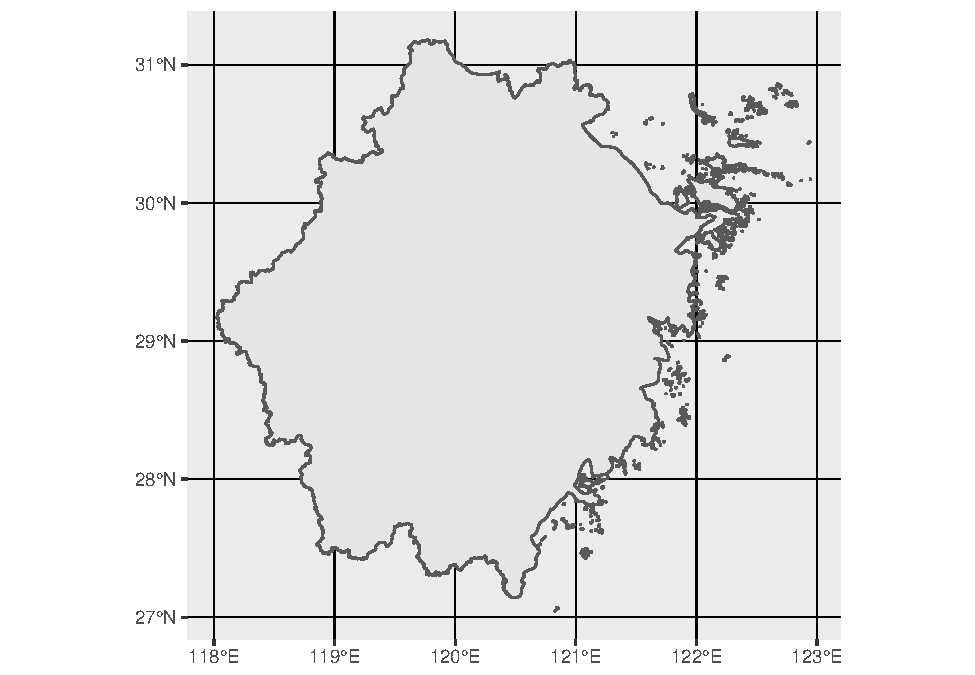
\includegraphics{利用高德地图API接口生成行政区划图_files/figure-latex/ggplot_zj-1} 

}

\caption{浙江省行政区图}\label{fig:ggplot_zj}
\end{figure}

\subsubsection{延伸}

通过以上的方法,我们可以一个行政区一个行政区的得到他们的边框,然后通过\texttt{rbind}得到更大区域的图了。然而,这样的方式是太low了。我们要充分利用R语言里的\texttt{apply}函数家族,一下子得到浙江省所有地级市的行政区图。直接上代码。

\begin{Shaded}
\begin{Highlighting}[]
\NormalTok{zj_city<-zj }\OperatorTok\StringTok{ "["}\NormalTok{(}\StringTok{'districts'}\NormalTok{) }\OperatorTok\StringTok{ '[['}\NormalTok{(}\DecValTok{1}\NormalTok{) }\OperatorTok\StringTok{ '[['}\NormalTok{(}\DecValTok{1}\NormalTok{)  }\CommentTok{#提取各城市adcode}
\NormalTok{zj_city<-}\KeywordTok{lapply}\NormalTok{(zj_city}\OperatorTok{$}\NormalTok{adcode,get_location)  }\OperatorTok\StringTok{         }\CommentTok{#利用lapply函数提取所有城市的地理信息}
\StringTok{         }\KeywordTok{list.map}\NormalTok{(districts) }\OperatorTok\StringTok{ }
\StringTok{         }\KeywordTok{lapply}\NormalTok{(select,}\OperatorTok{-}\NormalTok{districts) }\OperatorTok\StringTok{ }
\StringTok{         }\NormalTok{list.rbind}
\NormalTok{zj_city}\OperatorTok{$}\NormalTok{polyline <-}\StringTok{ }\NormalTok{zj_city}\OperatorTok{$}\NormalTok{polyline }\OperatorTok\StringTok{                    }
\StringTok{                    }\KeywordTok{str_split}\NormalTok{(}\StringTok{'}\CharTok{\textbackslash{}\textbackslash{}}\StringTok{|'}\NormalTok{) }\OperatorTok\StringTok{ }
\StringTok{                    }\KeywordTok{lapply}\NormalTok{(str_split,}\StringTok{';'}\NormalTok{) }\OperatorTok\StringTok{ }
\StringTok{                    }\KeywordTok{lapply}\NormalTok{(lapply,str_split,}\StringTok{','}\NormalTok{) }\OperatorTok
\StringTok{                    }\KeywordTok{lapply}\NormalTok{(lapply,lapply,as.numeric) }\OperatorTok\StringTok{ }
\StringTok{                    }\KeywordTok{lapply}\NormalTok{(lapply,list.rbind) }\OperatorTok
\StringTok{                    }\KeywordTok{lapply}\NormalTok{(lapply,gcj02_wgs84_matrix_matrix) }\OperatorTok\StringTok{ }
\StringTok{                    }\KeywordTok{lapply}\NormalTok{(lapply,list) }\OperatorTok
\StringTok{                    }\KeywordTok{lapply}\NormalTok{(st_multipolygon) }\OperatorTok\KeywordTok{st_sfc}\NormalTok{(}\DataTypeTok{crs=}\DecValTok{4326}\NormalTok{)}

\NormalTok{zj_city <-}\StringTok{ }\KeywordTok{st_sf}\NormalTok{(zj_city)}
\end{Highlighting}
\end{Shaded}

可以看出来,最后一段代码不过是又套了一层lapply而已。在这里我们先不着急出图,我们把各城市的名字标出来。位置就放在高德给出的城市中心位置,原汁原味吗。这里又要进行一下坐标的转换。

\begin{Shaded}
\begin{Highlighting}[]
\NormalTok{zj_city       <-zj_city}\OperatorTok{$}\NormalTok{center }\OperatorTok\StringTok{ }
\StringTok{                }\KeywordTok{str_split}\NormalTok{(}\StringTok{';'}\NormalTok{) }\OperatorTok\StringTok{ }
\StringTok{                }\KeywordTok{lapply}\NormalTok{(str_split,}\StringTok{','}\NormalTok{) }\OperatorTok\StringTok{ }
\StringTok{                }\KeywordTok{lapply}\NormalTok{(lapply,as.numeric) }\OperatorTok\StringTok{ }
\StringTok{                }\KeywordTok{lapply}\NormalTok{(list.rbind) }\OperatorTok\StringTok{ }\NormalTok{list.rbind }\OperatorTok\StringTok{ }
\StringTok{                }\NormalTok{gcj02_wgs84_matrix_df }\OperatorTok
\StringTok{                }\KeywordTok{bind_cols}\NormalTok{(zj_city)}
\NormalTok{zj_city<-}\KeywordTok{st_sf}\NormalTok{(zj_city)}
\end{Highlighting}
\end{Shaded}

我们来检验一下最终成果吧。

\begin{Shaded}
\begin{Highlighting}[]
\KeywordTok{library}\NormalTok{(showtext)}
\end{Highlighting}
\end{Shaded}

\begin{verbatim}
## Loading required package: sysfonts
\end{verbatim}

\begin{verbatim}
## Loading required package: showtextdb
\end{verbatim}

\begin{Shaded}
\begin{Highlighting}[]
\KeywordTok{showtext_auto}\NormalTok{()                  }\CommentTok{#由于ggplot2对中文支持不友好,这里需要加载一个显示中文的包}
\KeywordTok{ggplot}\NormalTok{() }\OperatorTok{+}\StringTok{ }\KeywordTok{geom_sf}\NormalTok{(}\DataTypeTok{data=}\NormalTok{zj_city) }\OperatorTok{+}\KeywordTok{geom_text}\NormalTok{(}\DataTypeTok{data=}\NormalTok{zj_city,}\KeywordTok{aes}\NormalTok{(}\DataTypeTok{x=}\NormalTok{wgs84_lng,}\DataTypeTok{y=}\NormalTok{wgs84_lat,}\DataTypeTok{label=}\NormalTok{name))}
\end{Highlighting}
\end{Shaded}

\begin{figure}

{\centering 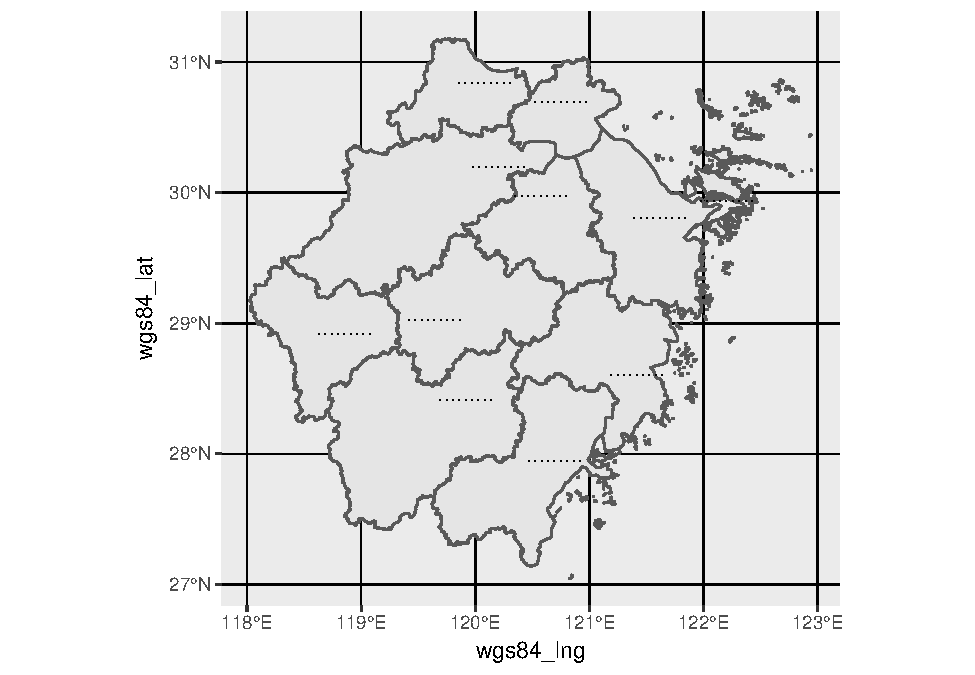
\includegraphics{利用高德地图API接口生成行政区划图_files/figure-latex/city_map-1} 

}

\caption{浙江省分市行政区划图}\label{fig:city_map}
\end{figure}


\end{document}
